% [5~v\textsuperscript{o}]
\pstart%
Postea resectis arteriis et auriculis plane utrinque
\edtext{[discissis]}{\lemma{disscissis}\Bfootnote{\textit{L \"{a}ndert Hrsg.}}}
clare cognovi quomodo valvula ex cava ad arteriam venosam esset disposita, nempe tali modo, ut recta ex cava sanguis in extremitatem auriculae sinistrae ingrederetur atque inde postea tum ad pulmones tum in \edtext{sinum}{\lemma{}\Bfootnote{sinum \textbar\ sinum \textit{gestr.}\ \textbar\ sinistrum \textit{L}}} sinistrum regurgitaret; ita tamen ut nihil omnino per illam ex sinistra parte in dextrum sinum regredi posset.
\pend%
%\vspace*{1.5em}%
\pstart%
% \begin{wrapfigure}{l}{0.5\textwidth}
% \caption{Bildbeschreibung}
% \end{wrapfigure}
Inspexi deinde in basi, vasis resectis qualia essent eorum orificia; erantque ut ibi appinxi. $a$ est cava, $b$ arteria venosa, $c$ vena arteriosa, in medio est aorta cujus valvula inter $c$ et $a$ vix poterat aperiri aliae duae semper patebant, ideoque arteria venosa ibi erat inflexa, nec nisi duas valvulas habitura ex quibus unica erat formata, qua sola ab aorta separabatur; alia autem vasa omnia satis crasso interstitio ab invicem sejungebantur,
\edtext{(+~margini ascripta~+) imo istae rugae erant pars auriculae quam eo intus depresserat ut appareret totum cor a cava esse factum ex eadem materia ex qua auriculae cum tamen paulatim ejus tunica durior evaderet: non autem cordis caro quod non ita alluebatur humore intus transeunte, et ideo cavae et valvulae ex ea videbantur diversae naturae quam cor.}{\lemma{(\phantom)\hspace{-1.2mm}+~margini [...]}\Bfootnote{cor. \textit{erg. L}}}
$dbc$ est sinus sinister[,] $dace$ dexter[,] circuitus cavae in $a$ erat intus rugosus, \setline{6}caro cordis in $c$ ad venam arteriosam magis prominebat quam in caeteris locis.
\pend%
\vspace{1.5em}%
\pstart%
\centering%
\noindent%
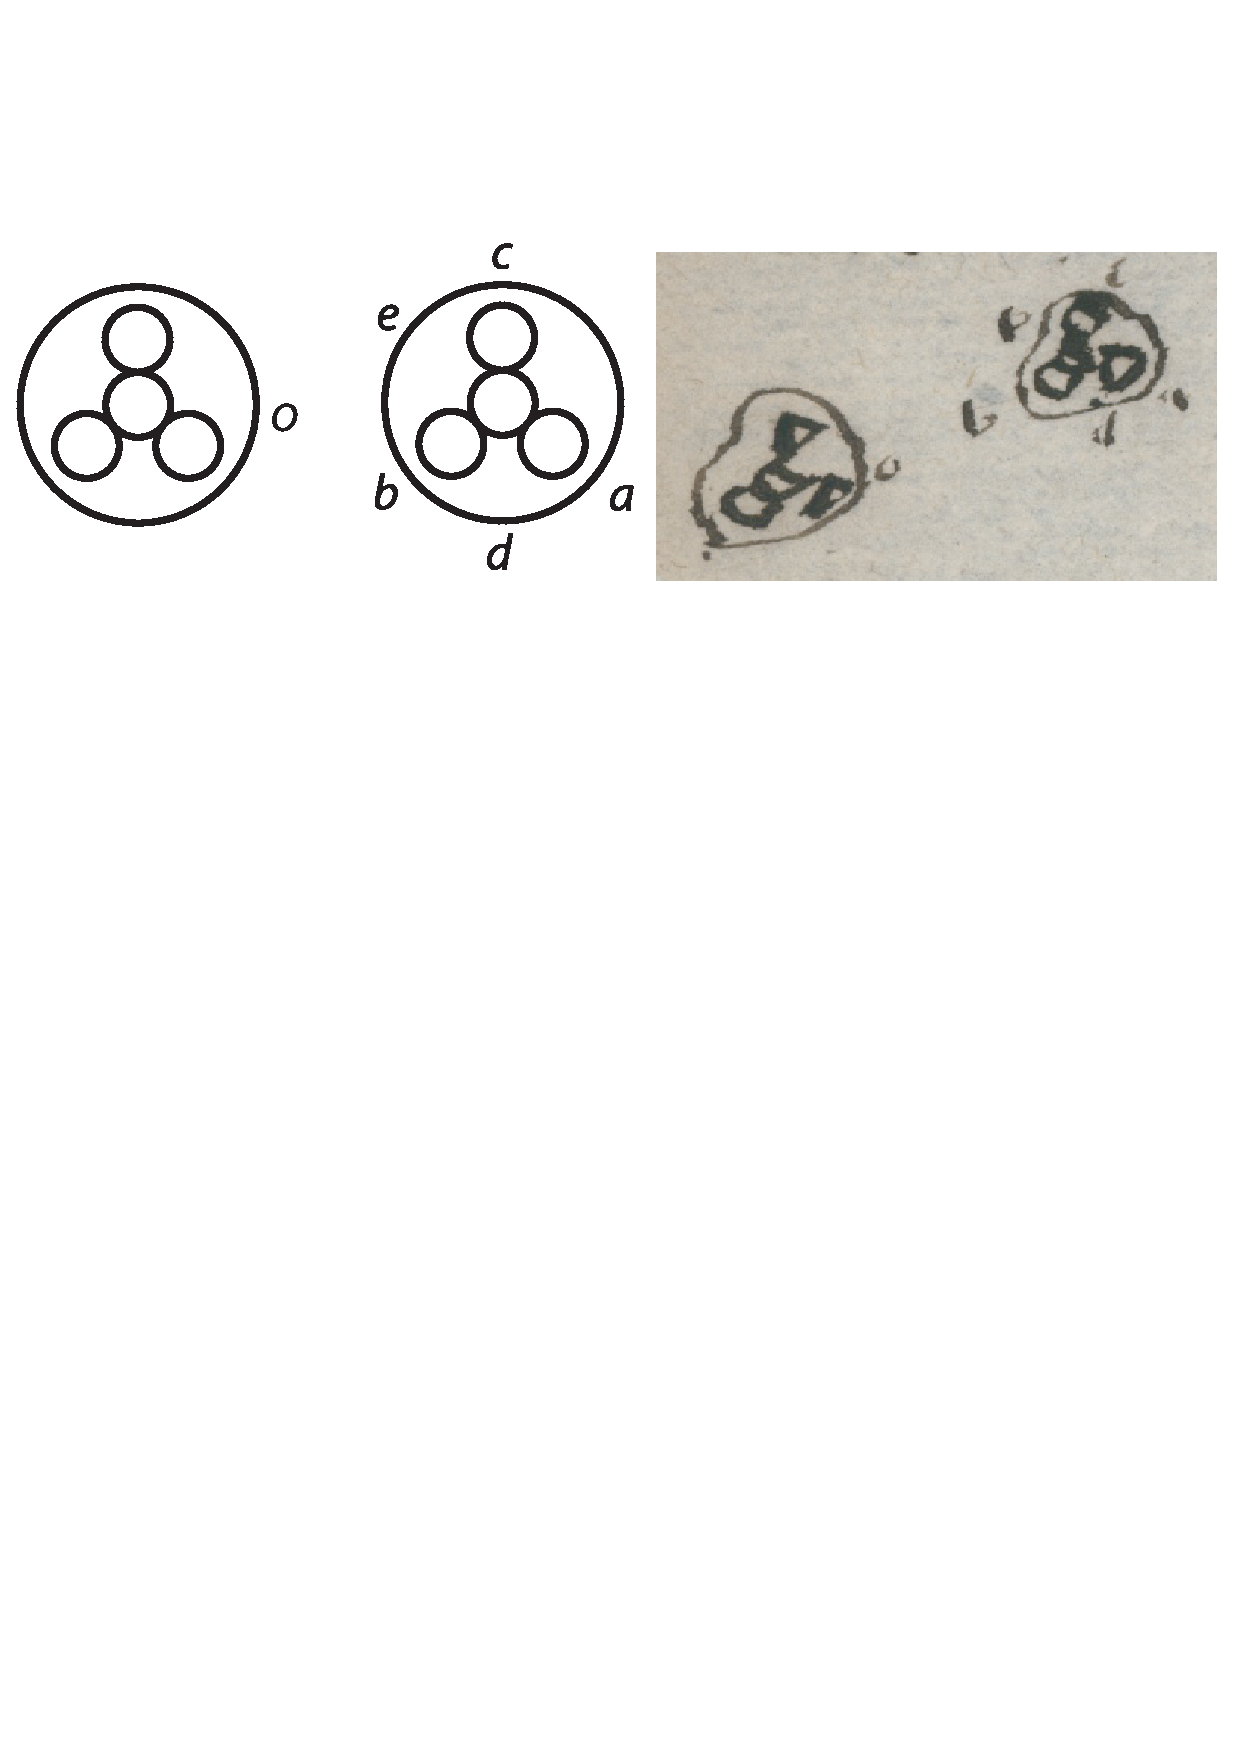
\includegraphics[trim = 0mm -3mm 0mm 0mm, clip, width=0.73\textwidth]{images/lh0040104b_005v1.pdf}\\
\centering [\textit{Fig. 7}]
\pend%
\vspace{1.5em}%
\pstart%
Secui \setline{5}deinde mucronem cordis illumque reperi tantum in aorta et vena arteriosa perforatum, erat autem foramen plane corrugatum intus tanquam vesica manu pressa, et poterat everti tanquam auricula planeque ejusdem fabricae intus videbatur, nec caro in summo mucrone magis crassa erat: eminebant vero ex eo fibrae quaedam albae quae retis instar intertextae et prominentiis in sinus cavitate existentibus adhaerebant sursum versus; erant vero tantum istae fibrae versus aortam.
\pend
\pstart%
\begin{wrapfigure}[10]{l}{0.46\textwidth}
\vspace{-4mm}\includegraphics[trim = 1mm 0mm -3mm -5mm, clip,width=0.46\textwidth]{images/lh0040104b_005v3.pdf}\\
\centering [\textit{Fig. 8}]
%\caption{Bildbeschreibung}
\end{wrapfigure}
Secui deinde eundem mucronem paulo altius ubi perspicue vidi foramen ab aorta et arteria venosa esse rotundum a venis vero oblongum; et illum amplectens ut $abc.$ Incipiebant vero etiam fibrae esse in sinistro sinu versus arteriam venosam.
Secui deinde cavam in $a$ a basi ad mucronem per exterius apparentia sinuum interstitia, et eodem modo venam arteriosam in $b,$ mansitque totus ventriculus $aeb$ expansus, ita \edtext{ut tamen}{\lemma{ita}\Bfootnote{\textit{(1)}\ tantum \textit{(2)}\ ut tamen \textit{L}}} appareret intermedia $fe$ et columna intra $fe$ sita[,]
de qua supra[,] cujus basis erat $ce,$ \edtext{(+~margini ascripta~+) exterius inferiori parti istius columnae quasi basis alterius adjuncta erat ex quo fibrae dividentes valvulas cavae in $o$ veniebant}{\lemma{(\phantom)\hspace{-1.2mm}+~margini [...] veniebant}\Bfootnote{\textit{erg. L}}} aut circiter, carnis autem densitas circumquaque fere aequalis et quamvis oblique secta non tamen erat latior quam
$gh.$ Aperui denique arteriam venosam in sui medio nempe $cd$ et scidi membranam $f$ inter arterias positam potuitque totus sinus repraesentari ut pictum est, et manifestum erat, hunc sinum ita angustum esse, quia fuerat a dextro compressum: ejus autem caro ubique aequaliter densa duplo aut circiter densior quam alterius non tamen multo latior sed compactior; nec vero erat magis lata vel densa in medio pariete quam in reliquis adeo ut videretur sinus quidem hic sinister fuisse quidem inflatus et rotundus eique postea superaccrevisse sinus dexter tanquam operculum. Notandum etiam aperto sinu sinistro per medium arteriae venosae $dc$ tantum potuisse explicari priusquam valvula $f$ scinderetur atque post; adeo ut ora venarum essent multo laxiora quam arteriarum nempe cavae orificium erat omnium latissimum; minimum erat aortae, reliqua duo fere aequalia.
\pend%
\vspace{1.0em}% PR: Bitte diesen leeren Zeilenabstand behalten !!!
\pstart%
\noindent% PR: Neuer Abschnitt.
In bove animadverti cavum cui implantatus fuerat umbilicus, non amplius crassiuscula carne circumvallatum sed plane acuminata, recedebatque a felle 4 digitorum distantia erat hepatis caro magis colorata quam vitulorum, pulmonum vero minus, sed plane albicans.
\pend
\pstart
Duae tamen apparebant insignes et nigricantes venae cutaneae cordis, utraque ab eadem origine ortum ducebat nempe a ramo insigni cavae, qui per medium parietem cordis ab ingressu cavae ad auriculam sinistram pervadens ibi 1\textsuperscript{mo} bifariam dividebatur interjecta valvula ejusque ramus inferior rursus bifariam divisus unam sui partem perpendiculariter ad mucronem cordis descendentem supra medium sinistri sinus emittebat. Altera oblique infra sinistram auriculam serpens postquam ad ejus finem pervenerat versus mucronem cordis in separatione utriusque sinus anterius flectebatur; alius vero ramus istius venae omnium maximus supra sinistram auriculam serpens sursum ascendebat et juxta illam nervulus descendebat versus cor, qui tamen in pericardio videbatur absumi ut et alii nervi quotcunque mihi occurrerunt; notavi praeterea valvulis claudi orificia venae azygos et axillaris quae a cavae ascendentis trunco veniebat, ita ut sanguis per illas facilius versus cor laberetur quam inde posset regredi. In arteriis autem nulla prorsus ejusmodi valvularum vestigia apparebant: ipsae autem cordis valvulae erant ut in vitulis nempe
\edtext{cavae et}{\lemma{}\Bfootnote{cavae \textbar\ nempe cavae \textit{gestr.}\ \textbar\ et \textit{L}}}
arteriae venosae minus perfectae, venae autem perfectissimae, aortae perfectae quidem, sed quae tamen non tam plane claudebantur quam vena arteriosa: hujusque orificium proportione minus erat quam in vitulis aortae majus.
\pend%
\pstart%
Ex duobus ramulis aortae immediate supra valvulas egredientibus sinister deorsum ad mucronem cordis anterius inter utrumque sinum simul cum vena flectebatur; dexter oblique serpens infra
\edtext{dextram [auriculam]}{%
\lemma{dextram}\Bfootnote{%
\textit{(1)}\ auriculae partem %
\textit{(2)}\ auriculae paulatim
\textit{L ändert Hrsg.}}}
paulatim in cor absumebatur, quatuor exiguis ramulis statim ab initio in cor demissis.
Sed et sinister ramus cujus tamen unam partem
\pend
\newpage
\pstart\noindent jamjam \edtext{descripsi}{\lemma{descripsi}\Cfootnote{Siehe oben, % LH IV 1,4B Bl. 3~v\textsuperscript{o}, Z. 24ff, hier 
S. \pageref{ramus}.}}
unicum praeterea ramulum in ipso initio in cor demittens maxima sui parte infra sinistram auriculam ad principium cavae usque serpebat,
[6~r\textsuperscript{o}]
atque ibi versus cordis mucronem deflexa sinum dextrum a sinistro in posteriore cordis superficie distinguebat.
\pend%
%\count\Bfootins=1500
%\count\Cfootins=1500
%\count\Afootins=1500